\chapter{Estrazione RNA con kit su colonnina Qiagen e retrotrascrizione in cDNA} % Title

\section{Sommario}

\subsection{Scopo}
Lo scopo di quest'esperienza è l'estrazione dell'RNA e la retrotrascrizione dell'RNA in cDNA. \\
L'RNA estratto appartiene a cellule di melanoma umane.

\subsection{Cenni teorici}

L'RNA è formato dagli acidi nucleici, cioè grosse molecole in cui è depositata
l'informazione genetica: detto in parole povere, le "istruzioni" in essi contenute
vengono decodificate attraverso una serie di reazioni biochimiche per "creare" le varie proteine dell'organismo.
Grazie all'analisi del materiale genetico si possono ricavare una serie di informazioni utili per molte analisi mediche.

\section{Materiali utilizzati}

\begin{itemize}
\item Guanti in lattice
\item Micropipette (\SI{100}{\micro\liter}-\SI{1000}{\micro\liter} e \SI{2}{\micro\liter}-\SI{200}{\micro\liter})
\item Eppendorf da 1,5mL
\item Eppendorf da \SI{200}{\micro\liter} pulita
\item Collection tube pulito
\end{itemize}

\section{Soluzioni utilizzate}

\begin{itemize}

\item Eppendorf di RTL Buffer( \SI{350}{\micro\liter} )
\item Eppendorf di etranolo 70\%, marchiata ET
\item Eppendorf di RW1 Buffer (\SI{700}{\micro\liter})
\item Eppendorf di RPE Buffer (\SI{1000}{\micro\liter}); servirà per due passaggi da \SI{500}{\micro\liter} cad.
\item Eppendorf da \SI{200}{\micro\liter} con RNAse-free H2O
\item Eppendorf da 1,5ml RNAse-free
\end{itemize}

\subsection{Funzioni delle soluzioni}

\begin{itemize}

\item RTL : il Buffer RLT è un tampone per la lisi di cellule e tessuti prima
dell'isolamento dell'RNA e di quello simultaneo di  RNA, DNA e proteine.
Esso contiene sali di guanidina istocinato.

\item RW1: Il tampone RW1 contiene un sale di guanidina ed è usato come un tampone
di lavaggio stringente che rimuove efficacemente le biomolecole come carboidrati, proteine, acidi grassi ecc.
Allo stesso tempo, molecole di RNA più grandi di 200 basi rimangono legate alla colonna.
Il tampone RW1 non deve essere usato per l'isolamento di piccoli RNA, per esempio microRNA o
RNA frammentato da tessuti fissati in formalina, poiché
questi frammenti più piccoli verranno lavati via.

\item RPE: Buffer RPE è un tampone di lavaggio delicato.
La sua funzione principale è quella di rimuovere le tracce di sali,
che sono ancora sulla colonna a causa dei buffer utilizzati in precedenza nel protocollo.
L'etanolo, che viene aggiunto dall'utente appena prima di usare il kit per la prima volta,
è un ingrediente importante di Buffer RPE.

\item RNAse-free: acqua senza enzimi RNAsi che degradano l'RNA
\end{itemize}

\section{Procedimento}

\subsection{Estrazione dell'RNA dal pellet cellulare}
\begin{enumerate}

\item Risospendere accuratamente le cellule con \SI{350}{\micro\liter} di RTL
utilizzando un puntale da \SI{1000}{\micro\liter}, pipettando più volte,
sino ad ottenere una sospensione(non aderente) omogenea.
Aggiungere RTL per permettere la lisi delle cellule,
così da permettere il rilascio del contenuto nucleare.
\item Aggiungere \SI{350}{\micro\liter} di etanolo \%70 alla sospensione e miscelare.
L'etanolo rende L'RNA meno solubile in acqua e aiuta la separazione in diverse fasi durante la centrifuga.
\item Spostare tutti i \SI{700}{\micro\liter} sulla colonnina rosa del kit,
montata sul suo collection tube.
Questa colonnina serve da filtro per l'RNA, infatti l'RNA rimane legato alla
membrana di colonnina, che è composta da silice.
L'RNA resta legato alla membrana fino a quando non si aggiunge l'H$_2$O.
\item Centrifugare a 8000 g per 15'', in modo da eliminare lo scarto.
\item Eliminare, smontando la colonnina, l'eluato, cioè quello che è passato attraverso la matrice.
\item Rimontare la colonnina sul collection tube.
\item Aggiungere \SI{700}{\micro\liter} di RW1 sulla colonnina.
In questa fase viene usato l'RW1 per lavare l'RNA dall'etanolo aggiunto in precedenza,
visto che ora non serve.
\item Centrifugare a 8000 g per 15''.
\item Eliminare, smontando la colonnina, l'eluato.
\item Aggiungere  \SI{500}{\micro\liter} di RPE sulla colonnina.
L'RPE, in questa fase, elimina le impurità rimaste nell'RNA.
\item Centrifugare a 8000 g per 2'.
\item Eliminare, smontando la colonnina, l'eluato.
\item Rimontare la colonnina sul nuovo collection tube fornito.
\item Centrifugare a massima velocità per 1', in quanto l'etanolo va eliminato completamente.
\item Eliminare il collection tube; porre la colonnina su eppendorf da 1,5 ml RNAse-free e
aggiungere \SI{30}{\micro\liter} di RNAse-free H$_2$O sulla colonnina,
così da non degradare l'RNA.
L'acqua inserita è senza enzimi che altrimenti degraderebbero l'RNA.
\item Centrifugare a 8000 g per 1'.\\
N.B: attenzione a come si inserisce l'eppendorf nella centrifuga, poich\`e se la si posiziona storta
il tappo potrebbe venir tranciato dalla centrifuga. per questo si consiglia di farsi aiutare da un esperto.
\item Ora l'RNA estratto è sul fondo della eppendorf.
L'H$_2$O è pi\`u affine all'RNA rispetto alla matrice
quindi centrifugando porta l'RNA sul fondo della eppendorf.

\end{enumerate}
%inserire immagini

\subsection{Quantificazione RNA estratto}

\begin{table}[H]
\begin{center}

\caption{Risultati di quantificazione al NanoDrop.}
\vspace{0,3cm}
\begin{tabular}{lrrrrr}
   & \multicolumn{1}{c}{Risultati al Nanodrop} \\
   Esame & \multicolumn{1}{c}{I} \\ \hline
    & & & & & \\

  A260 /A280 & $0,71$  \\
 A260/A230 & $1,97$   \\
  ng/uL & $52,7$   \\ \\ \hline
       & & & & & \\
  & & & & &  \\ \multicolumn{6}{l}{\small Fonte: Dati dal laboraorio}
\end{tabular}

\end{center}
\end{table}
Dopo aver quantificato al NanoDrop aliquotare \SI{8}{\micro\liter} su una eppendorf da \SI{200}{\micro\liter} pulita.

\subsection{Commento dei risultati}
Il nanodrop restituisce la concentrazione del campione in ng/$\mu$l e la sua purezza rispetto
a proteine e solventi organici o carboidrati, calcolata dal rapporto 260/280 e 260/230.
Il calcolo per trovare l'RNA estratto deriva dalla moltiplicazione della concentrazione del
campione per i microlitri di RNA, cioè sono stato estratti \SI{1,5}{\micro\gram} di RNA.
Dai dati è emerso che la purezza dell'RNA rispetto ai solventi organici è di $0,71$.
Per una buona purezza dovrebbe essere intorno a $2$, questo vuol dire
che c'è stato un errore nella centrifugazione oppure è rimasto troppo etanolo.

\subsection{Retrotrascrizione dell'RNA in cDNA}
\begin{enumerate}

\item Utilizzare l'RNA aliquotato in precedenza.
\item Denaturarlo a 65 °C per 10' nel termociclatore.
Così da permettere ad ogni singolo filamento di disappaiarsi$(fig1)$.
\item Spostare velocemente in ghiaccio i campioni.
In questo modo si denatura l'RNA grazie allo shock termico.
\item Aggiungere \SI{7}{\micro\liter} di mix (reagente di retrotrascrizione) al tubo con l'RNA
denaturato e miscelare pipettando.
\item Centrifugare brevemente i tubi,
in modo da trattenere la miscela di reazione sul fondo.
\item Per avviare la reazione \`e necessario portare i tubi a 37°C per 60'.
\item Conservare a -20\textcelsius

\begin{figure}[H]

\centering
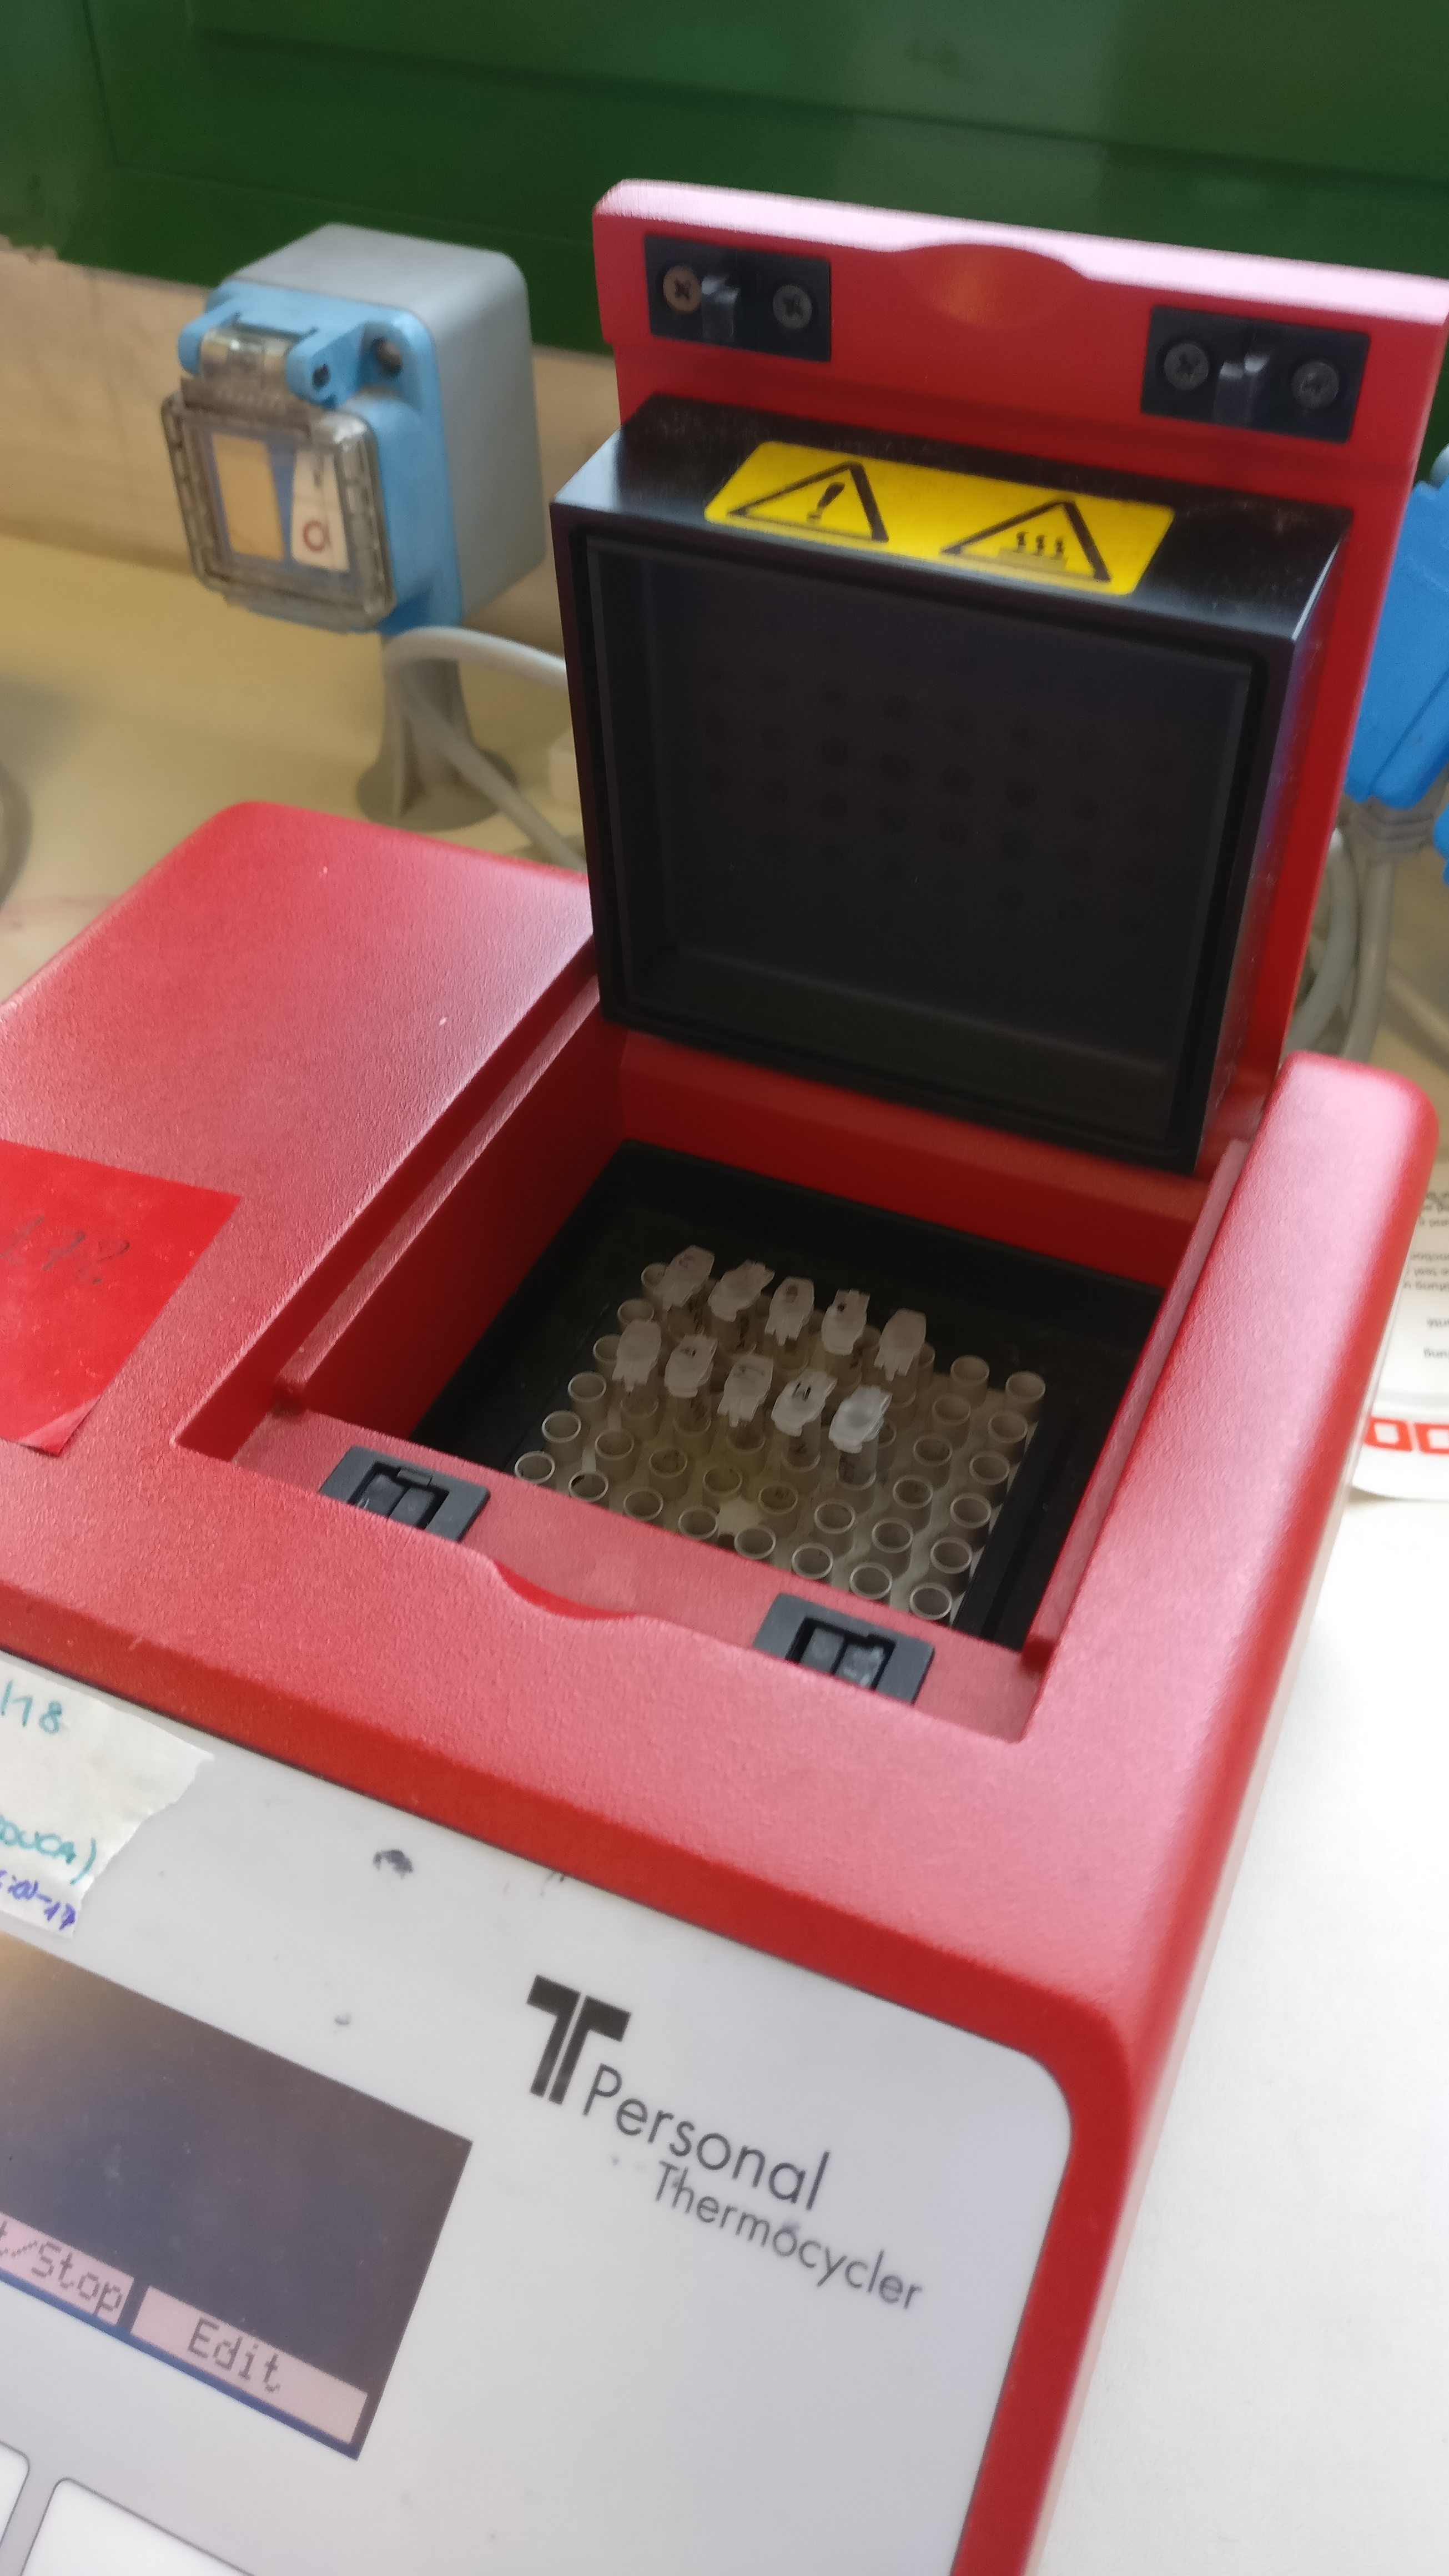
\includegraphics[width=0.3\textwidth]{./immagini/termociclatore.jpg}
\caption{eppendorf nel termociclatore}
\label{termociclatore}

\end{figure}

\end{enumerate}
